\documentclass{amsart}

\usepackage{tikz, lipsum}
\usetikzlibrary{positioning, decorations.pathreplacing, calc, arrows.meta, shapes.geometric}

\tikzset{
    bigbox/.style={draw, rounded corners, minimum width=2.5cm, minimum height=1.5cm},
    smallbox/.style={draw, rounded corners, minimum width=2cm, minimum height=1cm},
    bigcircle/.style={draw, circle, minimum size=2cm},
    bigellipse/.style={draw, ellipse, minimum width=3cm, minimum height=2.5cm},
    place/.style={inner sep=0pt, outer sep=0pt},
    fork/.style={decorate, decoration={show path construction, lineto code={
        \draw[rounded corners, ->](\tikzinputsegmentfirst)-|($(\tikzinputsegmentfirst)!.5!(\tikzinputsegmentlast)$)|-(\tikzinputsegmentlast);}
    }}
}

\begin{document}
\lipsum[1]
\[
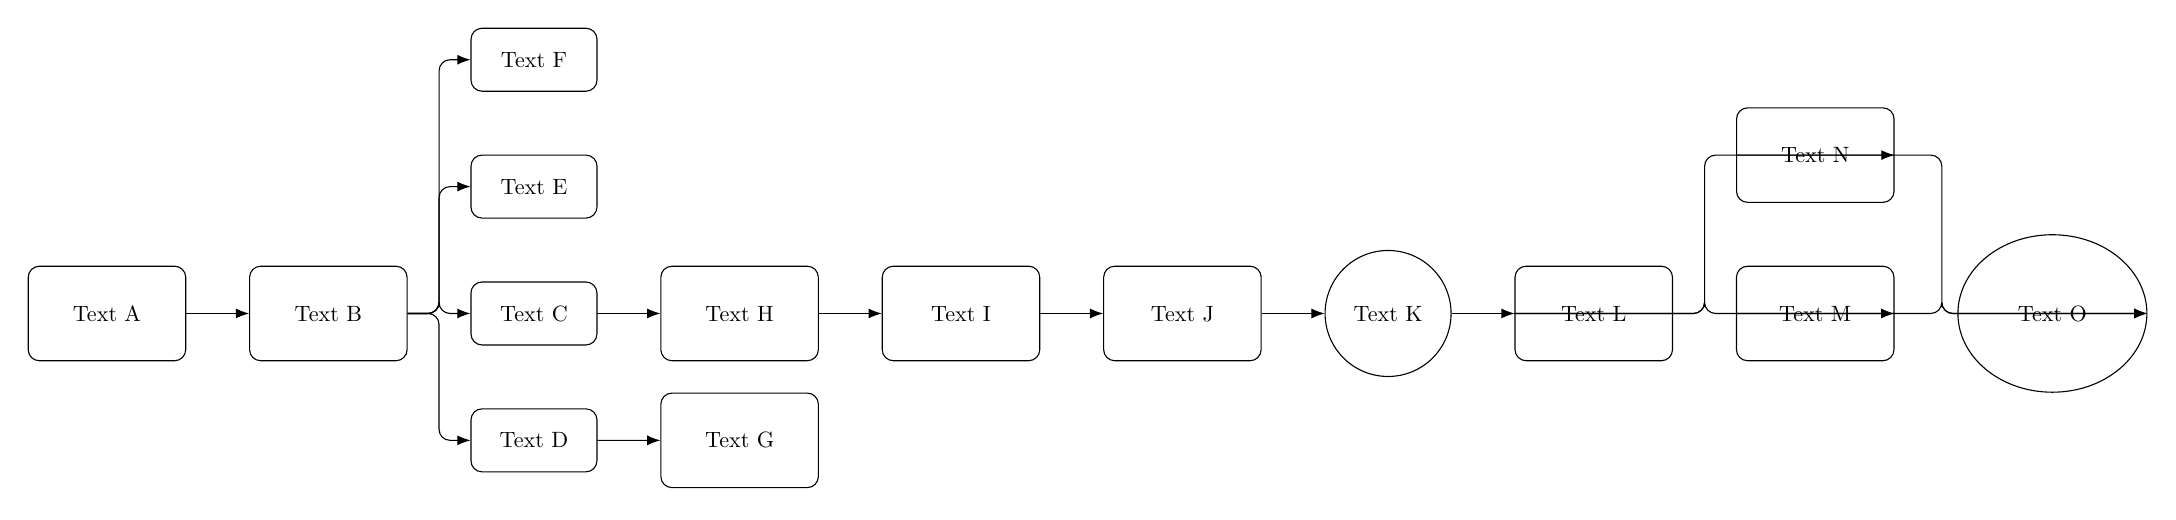
\begin{tikzpicture}[scale=.8, transform shape, node distance=1cm, >=Latex]
  \node(A)[bigbox]{Text A};
  \node(B)[bigbox, right=of A]{Text B};
  \node[place](X)[below=of A]{};
  \node(C)[smallbox, right=of B]{Text C};
  \node(D)[smallbox, below=of C]{Text D};
  \node(E)[smallbox, above=of C]{Text E};
  \node(F)[smallbox, above=of E]{Text F};
  \node(G)[bigbox, right=of D]{Text G};
  \node(H)[bigbox, right=of C]{Text H};
  \node(I)[bigbox, right=of H]{Text I};
  \node(J)[bigbox, right=of I]{Text J};
  \node(K)[bigcircle, right=of J]{Text K};
  \node(L)[bigbox, right=of K]{Text L};
  \node[place](Y)[below=of X]{};
  \node(M)[bigbox, right=of L]{Text M};
  \node(N)[bigbox, above=of M]{Text N};
  \node(O)[bigellipse, right=of M]{Text O};
  \draw[->](A)--(B);
  \draw[fork](B.east)--(D.west);
  \draw[fork](B.east)--(C.west);
  \draw[fork](B.east)--(E.west);
  \draw[fork](B.east)--(F.west);
  \draw[->](D)--(G);
  \draw[->](C)--(H);
  \draw[->](H)--(I);
  \draw[->](I)--(J);
  \draw[->](J)--(K);
  \draw[->](K)--(L);
  \draw[fork](L.west)--(M.east);
  \draw[fork](L.west)--(N.east);
  \draw[fork](M.west)--(O.east);
  \draw[fork](N.west)--(O.east);
\end{tikzpicture}
\]
\lipsum[2]
\end{document}
